 \let\negmedspace\undefined
\let\negthickspace\undefined
\documentclass[journal]{IEEEtran}
\usepackage[a5paper, margin=10mm, onecolumn]{geometry}
%\usepackage{lmodern} % Ensure lmodern is loaded for pdflatex
\usepackage{tfrupee} % Include tfrupee package

\setlength{\headheight}{1cm} % Set the height of the header box
\setlength{\headsep}{0mm}     % Set the distance between the header box and the top of the text
\usepackage{gvv-book}
\usepackage{gvv}
\usepackage{cite}
\usepackage{amsmath,amssymb,amsfonts,amsthm}
\usepackage{algorithmic}
\usepackage{graphicx}
\usepackage{textcomp}
\usepackage{xcolor}
\usepackage{txfonts}
\usepackage{listings}
\usepackage{enumitem}
\usepackage{mathtools}
\usepackage{gensymb}
\usepackage{comment}
\usepackage[breaklinks=true]{hyperref}
\usepackage{tkz-euclide} 
\usepackage{listings}
% \usepackage{gvv}                                        
\def\inputGnumericTable{}                                 
\usepackage[latin1]{inputenc}                                
\usepackage{color}                                            
\usepackage{array}                                            
\usepackage{longtable}                                       
\usepackage{calc}                                             
\usepackage{multirow}                                         
\usepackage{hhline}                                           
\usepackage{ifthen}                                           
\usepackage{lscape}



\usepackage{amsmath,amssymb}
\usepackage{booktabs}
\usepackage{tikz}
\usetikzlibrary{arrows.meta,angles,quotes}





\begin{document}

\bibliographystyle{IEEEtran}
\vspace{3cm}

\title{1.7.7}
\author{AI25BTECH11021 - Abhiram Reddy N}
% \maketitle
% \newpage
% \bigskip
{\let\newpage\relax\maketitle}

\renewcommand{\thefigure}{\theenumi}
\renewcommand{\thetable}{\theenumi}
\setlength{\intextsep}{10pt} % Space between text and floats


\numberwithin{equation}{enumi}
\numberwithin{figure}{enumi}
\renewcommand{\thetable}{\theenumi}


\textbf{Question}:\\For what value of p are the points (2, 1), (p, -1), and (-1, 3) collinear?


\textbf{Solution using Rank and RREF}

We are given the points
\[
A = (2,1), \quad B = (p,-1), \quad C = (-1,3).
\]

\textbf{Step 1: Vectors for Collinearity}
The points $A, B, C$ are collinear if the vectors 
\(\overrightarrow{AB}\) and \(\overrightarrow{AC}\) are linearly dependent.  

\[
\overrightarrow{AB} = (p-2, -2), \qquad 
\overrightarrow{AC} = (-3,2).
\]

\textbf{Step 2: Form Matrix}
We form a matrix $M$ with these vectors as rows:
\[
M = \begin{bmatrix}
p-2 & -2 \\
-3 & 2
\end{bmatrix}.
\]

For collinearity, the rank of $M$ must be $1$ (since the two rows are linearly dependent).

\textbf{Step 3: Row Reduction (Echelon Form)}
Perform row operations to reduce $M$ to echelon form.

\[
R_1 = \begin{bmatrix} p-2 & -2 \end{bmatrix}, 
\quad R_2 = \begin{bmatrix} -3 & 2 \end{bmatrix}.
\]

Eliminate the first element of $R_2$:
\[
R_2 \to R_2 + \frac{3}{p-2} R_1.
\]

\[
R_2 = \begin{bmatrix} -3 & 2 \end{bmatrix} 
+ \frac{3}{p-2}\begin{bmatrix} p-2 & -2 \end{bmatrix}
= \begin{bmatrix} -3 + 3 & 2 - \frac{6}{p-2} \end{bmatrix}
= \begin{bmatrix} 0 & \frac{2(p-2)-6}{p-2} \end{bmatrix}.
\]

\textbf{Step 4: Condition for Rank $=1$}
For rank to be $1$, the second row must vanish:
\[
\frac{2(p-2)-6}{p-2} = 0.
\]

\[
2(p-2) - 6 = 0 \quad \implies \quad 2p - 10 = 0.
\]

\[
\boxed{p = 5}
\]

\textbf{Step 5: Verification}
When $p=5$, the points are
\[
A = (2,1), \quad B = (5,-1), \quad C = (-1,3).
\]
The slope of $AB$ is
\[
\frac{-1-1}{5-2} = \frac{-2}{3},
\]
and the slope of $AC$ is
\[
\frac{3-1}{-1-2} = \frac{2}{-3} = \frac{-2}{3}.
\]
Since slopes are equal, $A,B,C$ are collinear.









\begin{figure}[htbp]
\centering
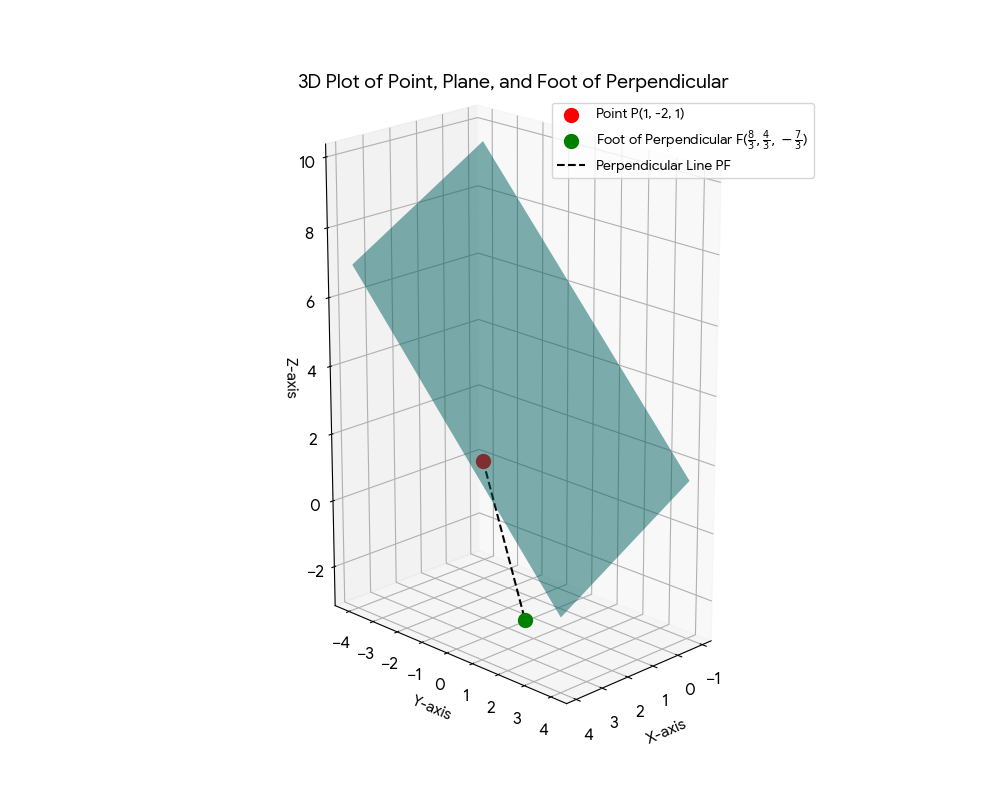
\includegraphics[width=0.8\columnwidth]{figs/python_plot.png} 
\caption{plot}
\label{fig:1}
\end{figure}
















\end{document}